%% \documentclass[handout,t]{beamer} % HANDOUT
%% \documentclass[handout,notes=show,t]{beamer} % NOTES
\documentclass[t]{beamer} % SLIDES
\usepackage{etex}

\usetheme{DSM}
\usepackage{beamer-tools-dsm}

%%
%% some useful macros: mathematical notation etc.
%%

%% abbreviations for logic symbols
\renewcommand{\implies}{\Rightarrow}
\newcommand{\equivalent}{\Leftrightarrow}

%% abbreviations for common number spaces
\newcommand{\setN}[1][]{\mathbb{N}_{#1}} % allows \setN and \setN[0]
\newcommand{\setZ}{\mathbb{Z}}
\newcommand{\setQ}{\mathbb{Q}}
\newcommand{\setR}{\mathbb{R}}

%% sets and (sub-)sets defined by condition
\newcommand{\set}[1]{\{#1\}}
\newcommand{\setdef}[2]{\set{#1\,|\,#2}}
\newcommand{\bigset}[1]{\bigl\{#1\bigr\}}
\newcommand{\bigsetdef}[2]{\bigset{#1\bigm|#2}}
\newcommand{\setscale}[1]{\left\{#1\right\}}
\newcommand{\setdefscale}[2]{\setscale{#1\left|\,#2\right.}}

%% absolute value and norm
\newcommand{\abs}[1]{\lvert #1\rvert}
\newcommand{\bigabs}[1]{\bigl\lvert #1\bigr\rvert}
\newcommand{\absscale}[1]{\left\lvert #1\right\rvert}
\newcommand{\norm}[2][]{\lVert #2\rVert_{#1}}
\newcommand{\bignorm}[2][]{\bigl\lVert #2\bigr\rVert_{#1}}
\newcommand{\normscale}[2][]{\left\lVert #2\right\rVert_{#1}}

%% complement set (with optional index)
\newcommand{\compl}[1][]{\mathcal{C}^{#1}}

%% power set: \powerset{\Sigma^*}
\newcommand{\powerset}[1]{\mathcal{P}(#1)}

%% uparrow: a \ua b = direct dominance in ordered tree
\newcommand{\ua}{\uparrow}

%% left-right arrow: this $\lra$ that
\newcommand{\lra}{\leftrightarrow}

%% expanded engineering notation: 4.2\x\e+5
\newcommand{\e}[2]{10^{\ifthenelse{\equal{#1}{+}}{}{#1}#2}}
\newcommand{\x}{\cdot}

%% arg max & min: \argmax_{x\in C}, \argmin_{x\in C}
\newcommand{\argmax}{\mathop{\text{arg~max}}}
\newcommand{\argmin}{\mathop{\text{arg~min}}}

%% infinitesimal elements: \dx, \dy = \dX{y}, \dz
\newcommand{\dX}[1]{\,\mathit{d{#1}}}
\newcommand{\dx}{\dX{x}}
\newcommand{\dy}{\dX{y}}
\newcommand{\dz}{\dX{z}}

%%% Local Variables: 
%%% mode: latex
%%% TeX-master: ""
%%% End: 
  % basic mathematical notation
%%
%% some macros for typesetting text
%%

%% \OPEN ... \CLOSE; \OPEN[np] ... \CLOSE[np]
%% bold large brackets for labelled bracketing notation
\newcommand<>{\OPEN}[1][]{\only#2{$\boldsymbol{\bigl[}\text{}_{\text{\raisebox{-2pt}{\textsc{#1}}}}$}}
\newcommand<>{\CLOSE}[1][]{\only#2{$\text{}_{\text{\raisebox{-2pt}{\textsc{#1}}}}\boldsymbol{\bigr]}$}}

%% \textgap ("_" representing missing letter)
\newcommand{\textgap}{\mbox{\hspace{.4pt}\texttt{\bfseries\secondary{\textunderscore}}\hspace{.4pt}}}

%% \textstar, \textast (math \star and \ast symbols in text mode, with some extra spacing)
\newcommand{\textstar}{$\mspace{.8mu}\star\mspace{.8mu}$}
\newcommand{\textast}{$\ast$}

%% $\p{\ctext{abc}}$ (cited text in mathematical equations, e.g. n-gram probabilities)
\newcommand{\ctext}[1]{\text{\textcite{#1}}}

%% $\p{\btext{abc}}$ (normal black text even in coloured math environment)
\newcommand{\btext}[1]{\text{\foreground{#1}}} 

%% text subscripts and superscripts (can be used in math and text mode)
\newcommand{\tsup}[1]{\ensuremath{^{\text{#1}}}}
\newcommand{\tsub}[1]{\ensuremath{_{\text{#1}}}}

%%% Local Variables: 
%%% mode: latex
%%% TeX-master: ""
%%% End: 
  % some useful macros for plain text
%%
%% some useful macros: statistical notation
%%

%% \p{X=k};  \pC{X=k}{Y=l};  \bigp{X_i = k};   \pscale{\frac{Z}{S^2}};
%% probability P(X=k) and conditional probability P(X=k|Y=l), also with larger or scaled parentheses
%% \p[\theta]{X=k};  \pC[\text{interpolated}]{X=k}{Y=l};  ...
%% with optional subscripts (for model probability, null probability, etc.)
\newcommand{\p}[2][]{\mathop{\mathrm{Pr}_{#1}}(#2)}
\newcommand{\pscale}[2][]{\mathop{\mathrm{Pr}_{#1}}\!\left(#2\right)}
\newcommand{\bigp}[2][]{\mathop{\mathrm{Pr}_{#1}}\bigl(#2\bigr)}
\newcommand{\pC}[3][]{\p[#1]{#2\,|\,#3}} 
\newcommand{\pCscale}[3][]{\pscale[#1]{#2\left|\,#3\right.\!}} 
\newcommand{\bigpC}[3][]{\bigp[#1]{#2\!\bigm|\!#3}} 

%% \Exp{X};  \Var{X};  \Exp[0]{X};  \Var[0]{X};  
%% \bigExp{X}; \bigVar{X}; \Expscale{X};  \Varscale{X};
%% expectation E[X] and variance V[X], expectation and variance under null hypothesis, 
%% and variants with largeer or scaled brackets
\newcommand{\Exp}[2][]{\mathrm{E}_{#1}[#2]}
\newcommand{\Var}[2][]{\mathop{\mathrm{Var}}_{#1}[#2]}
\newcommand{\bigExp}[2][]{\mathrm{E}_{#1}\!\bigl[#2\bigr]}
\newcommand{\bigVar}[2][]{\mathop{\mathrm{Var}}_{#1}\bigl[#2\bigr]}
\newcommand{\Expscale}[2][]{\mathrm{E}_{#1}\left[#2\right]}
\newcommand{\Varscale}[2][]{\mathop{\mathrm{Var}}_{#1}\left[#2\right]}

%% \pihat = \hat{\pi}
%% sampling estimate for population probability \pi (may need fine-tuning)
\newcommand{\pihat}{\hat{\pi}}

%% \Entropy{X}, \Entropy{p}, \KL{p}{q}, \MI{X}{Y}
%% \bigEntropy{}, \Entropyscale{}, \bigKL{}{}, \KLscale{}{}, \bigMI{}{}, \MIscale{}{}
%% entropy, KL distance, conditional entropy and mutual information (with scaled variants)
\newcommand{\Entropy}[1]{H[{#1}]}
\newcommand{\bigEntropy}[1]{H\bigl[{#1}\bigr]}
\newcommand{\Entropyscale}[1]{H\left[{#1}\right]}
\newcommand{\KL}[2]{D({#1}\|{#2})}
\newcommand{\bigKL}[2]{D\bigl({#1}\bigm\|{#2}\bigr)}
\newcommand{\KLscale}[2]{D\left({#1}\left\|{#2}\right.\right)}
\newcommand{\MI}[2]{I[{#1};{#2}]}
\newcommand{\bigMI}[2]{I\bigl[{#1};{#2}\bigr]}
\newcommand{\MIscale}[2]{I\left[{#1};{#2}\right]}

%% \corr (correlation) and \cov (covariance) as mathop's
\newcommand{\corr}{\mathop{\mathrm{corr}}}
\newcommand{\cov}{\mathop{\mathrm{cov}}
}
%%% Local Variables: 
%%% mode: latex
%%% TeX-master: ""
%%% End: 
  % notation for probability theory and statistics
%%
%% convenience macros for linear algebra (vectors and matrices)
%%

%% \Vector[i]{x} ... vector variable with optional _superscript_ index in parentheses
%% \Vector[']{x} ... special case: ' superscript not enclosed in parentheses
%% \vx, \vy, \vz ... abbreviations for common vector names
\newcommand{\Vector}[2][]{\mathbf{#2}\ifthenelse{\equal{#1}{}}{}{^{(#1)}}}
\newcommand{\vx}[1][]{\Vector[#1]{x}}
\newcommand{\vy}[1][]{\Vector[#1]{y}}
\newcommand{\vz}[1][]{\Vector[#1]{z}}
\newcommand{\vu}[1][]{\Vector[#1]{u}}
\newcommand{\vv}[1][]{\Vector[#1]{v}}
\newcommand{\vw}[1][]{\Vector[#1]{w}}
\newcommand{\va}[1][]{\Vector[#1]{a}} % vectors of coefficients
\newcommand{\vb}[1][]{\Vector[#1]{b}} % for basis
\newcommand{\vc}[1][]{\Vector[#1]{c}} % context vectors
\newcommand{\ve}[1][]{\Vector[#1]{e}} % for standard basis of R^n
\newcommand{\vm}[1][]{\Vector[#1]{m}} % row vectors of term-term matrix
\newcommand{\vn}[1][]{\Vector[#1]{n}} % normal vector
\newcommand{\vmu}[1][]{\Vector[#1]{\boldsymbol{\mu}}} % column vectors of term-term matrix
\newcommand{\vf}[1][]{\Vector[#1]{f}} % row vectors of term-context matrix
\newcommand{\vphi}[1][]{\Vector[#1]{\boldsymbol{\phi}}} % column vectors of term-context matrix
\newcommand{\vxi}[1][]{\Vector[#1]{\boldsymbol{\xi}}} % coordinate vector
\newcommand{\vnull}[1][]{\Vector[#1]{0}} % neutral element

%% \Span{\vb[1],\ldots,\vb[k]} ... span of set of vectors
%% \Rank{...} ... rank of set of vectors or matrix
%% \Det{...}, \det A ... determinant of a set of vectors / a matrix A
%% \Image{f}, \Kernel{f} ... image and kernel of a linear map
\newcommand{\Span}[1]{\mathop{\text{sp}}\left(#1\right)}
\newcommand{\Rank}[1]{\mathop{\text{rank}}\left(#1\right)}
\newcommand{\Det}[1]{\mathop{\text{Det}}\left(#1\right)}
%% \det is already defined in the standard library
\newcommand{\Image}[1]{\mathop{\text{Im}}\left(#1\right)}
\newcommand{\Kernel}[1]{\mathop{\text{Ker}}\left(#1\right)}

%% \dist[2]{\vx}{\vy} ... distance between two vectors (p-metric)
\newcommand{\dist}[3][]{d_{#1}\left(#2, #3\right)}
\newcommand{\bigdist}[3][]{d_{#1}\bigl(#2, #3\bigr)}

%% \sprod{\vu}{\vv} ... scalar product
\newcommand{\sprod}[2]{\left\langle #1, #2 \right\rangle}
\newcommand{\bigsprod}[2]{\bigl\langle #1, #2 \bigr\rangle}


%%% Local Variables: 
%%% mode: latex
%%% TeX-master: ""
%%% End: 
% convenience macros for vectors and matrices

%%%
%%% local configuration adjustments
%%%

%%% You can change pre-defined colours here, override built-in macros from the
%%% style definition and standard library, as well as define macros needed by
%%% all local documents.

%%% e.g. adjust counterpoint (dark green) for data projectors where greens are
%%% far too bright, as well as green component of light colour and pure green
%%% (of course, it's a better solution to adjust the gamma settings of your monitor)
%%
%% \definecolor{counterpoint}{rgb}{.1, .3, 0}
%% \definecolor{light}{rgb}{.45, .3, .55}
%% \definecolor{puregreen}{rgb}{0, .35, 0}

%% ----- extra packages we need to load

\usepackage{tikz}
\usepackage{alltt}              % code examples with nicely formatted comments
\usepackage{hieroglf}           % hieroglyph font for the archeology example
\usepackage{rotating}
\usepackage{multirow}

%% ----- general copyright message (authors may change between versions of the tutorial)
\newcommand{\dsmcopyright}{%
  Copyright \textcopyright\ 2009--2016 Evert, Lenci, Baroni \& Lapesa | 
  Licensed under CC-by-sa version 3.0}


%% ----- automatically show TOC reminder at beginning of each subsection
\AtBeginSubsection[]
{
  \begin{frame}
    \frametitle{Outline}
    \tableofcontents[current,currentsubsection]
  \end{frame}
}

%% ----- some useful macros for the SIGIL course

%% > plot(x,y)      \REM{this produces a scatterplot}
\newcommand{\REM}[2][\small]{\textsf{#1\color{primary}\# #2}}

\newenvironment{Rcode}[1][]{%
\setbeamercolor{block title}{fg=counterpoint,bg=counterpoint!15!white}%
\setbeamercolor{block body}{bg=counterpoint!5!white}\small%
\begin{block}{#1}\begin{alltt}\ungap[1]}{%
\ungap[1]\end{alltt}\end{block}}

%% nice colour for R output: \begin{Rout} .. \end{Rout}
%% -- ugly hack: I'm sure theres a better way to do this
\newenvironment{Rout}[1][\footnotesize]{%
  \begin{footnotesize}#1\color{secondary}\bfseries}{%
  \color{black}\mdseries\end{footnotesize}}

%% symbols for centroid vector and singular value matrix 
%% \newcommand{\vmu}[1][]{\boldsymbol{\mu}\ifthenelse{\equal{#1}{}}{}{^{(#1)}}}
\newcommand{\Msigma}{\boldsymbol{\Sigma}}

%% rotated column labels for table (to fit long text into narrow columns
\newcommand{\rotLabel}[2][60]{\begin{rotate}{#1}#2\end{rotate}}
 % local adjustments to configuration and macros

%%%%%%%%%%%%%%%%%%%%%%%%%%%%%%%%%%%%%%%%%%%%%%%%%%%%%%%%%%%%%%%%%%%%%%
%% Titlepage

\title[DSM Tutorial -- Part 4]{Distributional Semantic Models}
\subtitle{Part 4: Elements of matrix algebra}
\author[\textcopyright\ Evert/Lenci/Baroni/Lapesa]{%
  Stefan Evert\inst{1}\\
  {\footnotesize with  Alessandro Lenci\inst{2}, Marco Baroni\inst{3} and Gabriella Lapesa\inst{4}}}
\institute[CC-by-sa]{%
  \inst{1}Friedrich-Alexander-Universität Erlangen-Nürnberg, Germany\\
  \inst{2}University of Pisa, Italy\\
  \inst{3}University of Trento, Italy\\
  \inst{4}University of Stuttgart, Germany
}

\date[wordspace.collocations.de]{
  \href{http://wordspace.collocations.de/doku.php/course:start}{\primary{\small http://wordspace.collocations.de/doku.php/course:start}}\\
  \light{\tiny \dsmcopyright}}

\begin{document}

\showLogo
\frame{\titlepage}
\hideLogo

%%%%%%%%%%%%%%%%%%%%%%%%%%%%%%%%%%%%%%%%%%%%%%%%%%%%%%%%%%%%%%%%%%%%%%

\section*{Outline}
\frame{ 
  \frametitle{Outline}
  \tableofcontents
}

%%%%%%%%%%%%%%%%%%%%%%%%%%%%%%%%%%%%%%%%%%%%%%%%%%%%%%%%%%%%%%%%%%%%%%
\section{Matrix algebra}

%%%%%%%%%%%%%%%%%%%%%%%%%%%%%%%%%%%%%%%%%%
\subsection{Roll your own DSM}

\begin{frame}[fragile]
  \frametitle{Matrices and vectors}
  
  \ungap[1]
  \begin{itemize}
  \item $k\times n$ matrix $\mathbf{M}\in \setR^{k\times n}$ is a rectangular array of real numbers
    \[
    \mathbf{M} = 
    \begin{bmatrix}
      m_{11} & \cdots & m_{1n} \\
      \vdots & & \vdots \\
      m_{k1} & \cdots & m_{kn}
    \end{bmatrix}
    \]
  \item Each row $\mathbf{m}_i\in \setR^n$ is an $n$-dimensional vector
    \[
    \mathbf{m}_i = (m_{i1}, m_{i2}, \ldots, m_{in})
    \]
  \item Similarly, each column is a $k$-dimensional vector $\in \setR^k$
  \end{itemize}

\sbox{\Rbox}{\primary{$\mathbf{m}_2$}}\ungap[1]
\begin{Rcode}
> options(digits=3)
> M <- DSM_TermTerm$M
> M[2, ] \REM{row vector \usebox{\Rbox} for ``dog''}
> M[, 5] \REM{column vector for ``important''}
\end{Rcode} %$ Emacs
\end{frame}

\begin{frame}[fragile]
  \frametitle{Matrices and vectors}

  \ungap[1]
  \begin{itemize}
  \item Vector $\mathbf{x}\in \setR^n$ as single-row or single-column matrix
    \begin{itemize}
    \item $\mathbf{x} = \mathbf{x}^{TT} = n\times 1$ matrix (``vertical'')
    \item $\mathbf{x}^T = 1\times n$ matrix (``horizontal'')
    \item \h{transposition} operator $\cdot^T$ swaps rows \& columns of matrix 
    \end{itemize}
  \item<2-> We need vectors $\mathbf{r} \in \setR^k$ and $\mathbf{c} \in \setR^n$ of marginal frequencies
  \item<2-> Notation for cell $ij$ of co-occurrence matrix:
    \begin{itemize}
    \item $m_{ij} = O$ \ldots\ observed co-occurrence frequency
    \item $r_i = R$ \ldots\ row marginal (target)
    \item $c_j = C$ \ldots\ column marginal (feature)
    \item $N$ \ldots\ sample size
    \end{itemize}
  \end{itemize}

\begin{Rcode}
> r <- DSM_TermTerm$rows$f
> c <- DSM_TermTerm$cols$f
> N <- DSM_TermTerm$globals$N
> t(r)    \REM{``horizontal'' vector}
> t(t(r)) \REM{``vertical'' vector} 
\end{Rcode} %$
\end{frame}

\begin{frame}[fragile]
  \frametitle{Scalar operations}
  
  \begin{itemize}
  \item \h{Scalar} operations perform the same transformation on each element of a vector or matrix, e.g.\
    \begin{itemize}
    \item add / subtract fixed shift $\mu\in \setR$
    \item multiply / divide by fixed factor $\sigma\in \setR$
    \item apply function ($\log, \sqrt{\cdot}, \ldots$) to each element
    \end{itemize}
  \item Allows efficient processing of large sets of values
  \item<2-> Element-wise binary operators on matching vectors / matrices
    \begin{itemize}
    \item $\mathbf{x} + \mathbf{y}$ = \h{vector addition}
    \item $\mathbf{x} \odot \mathbf{y}$ = element-wise multiplication (\hh{Hadamard product})
    \end{itemize}
  \end{itemize}
  
\begin{Rcode}
> log(M + 1) \REM{discounted log frequency weighting}
> (M["cause", ] + M["effect", ]) / 2 \REM{centroid vector}
\end{Rcode}
\end{frame}

\begin{frame}[fragile]
  \frametitle{The outer product}
  
  \ungap[1]
  \begin{itemize}
  \item Compute matrix $\mathbf{E}\in \setR^{k\times n}$ of expected frequencies
    \[
    e_{ij} = \frac{r_i c_j}{N}
    \]
    i.e.\ \code{r[i] * c[j]} for each cell $ij$
  \item<2-> This is the \h{outer product} of $\mathbf{r}$ and $\mathbf{c}$
    \begin{center}
      \begin{tikzpicture}[every matrix/.style={fixed matrix=6mm, cell matrix=5mm, matrix of nodes}]
        \matrix [bmatrix, anchor=north west] 
        (r) at (0, 0) {
          $r_1$ \\
          $\scaleVdots$ \\
          $r_k$ \\
        } ;
        \matrix [nmatrix, below right={0mm and 2mm of r.north east}] 
        (dot) {
          $\cdot$ \\
        } ;
        \matrix [bmatrix, below right={0mm and 2mm of dot.north east}] 
        (c) {
          $c_1$ & $c_2$ & $\scaleCdots$ & $c_n$ \\
        } ;
        \matrix [nmatrix, below right={0mm and 2mm of c.north east}] 
        (eq) {
          {} \\
          $=$ \\
        } ;
        \begin{scope}[every matrix/.append style={column sep={8mm,between origins}}]
          \matrix [bmatrix=2pt, column sep=1cm, below right={0mm and 2mm of eq.north east}] 
          (cross) {
            $r_1 c_1$ & $r_1 c_2$ & $\scaleCdots$ & $r_1 c_n$ \\
            $\scaleVdots$ & $\scaleVdots$ & & $\scaleVdots$ \\
            $r_k c_1$ & $r_k c_2$ & $\scaleCdots$ & $r_k c_n$ \\
          } ;
        \end{scope}
      \end{tikzpicture}
    \end{center}
  \item<3-> The \hh{inner product} of $\mathbf{x}, \mathbf{y}\in \setR^n$ is the sum $x_1 y_1 + \ldots + x_n y_n$
  \end{itemize}

\begin{Rcode}
> outer(r, c) / N
\end{Rcode}
\end{frame}

%%%%%%%%%%%%%%%%%%%%%%%%%%%%%%%%%%%%%%%%%%
\subsection{Matrix multiplication}

\begin{frame}
  \frametitle{Matrix multiplication}
  %% \framesubtitle{}

  \ungap
  \[
  \begin{array}{ccccc}
    \begin{bmatrix}
      & \only<beamer:2| handout:0>{a_{ij}} & \only<beamer:1| handout:0>{a_{ij}} & \\
      \only<beamer:3| handout:1>{a_{ij}} & & & \\
      & & &
    \end{bmatrix}
    & = &
    \begin{bmatrix}
      \only<beamer:1-2| handout:0>{b_{i1}} & \only<beamer:1-2| handout:0>{\cdots} & \only<beamer:1-2| handout:0>{b_{in}} \\
      \only<beamer:3| handout:1>{b_{i1}} & \only<beamer:3| handout:1>{\cdots} & \only<beamer:3| handout:1>{b_{in}} \\
      & &  
    \end{bmatrix}
    & \cdot &
    \begin{bmatrix}
     \only<beamer:3| handout:1>{c_{1j}}   & \only<beamer:2| handout:0>{c_{1j}} & \only<beamer:1| handout:0>{c_{1j}} &\\
     \only<beamer:3| handout:1>{\vdots}   & \only<beamer:2| handout:0>{\vdots} & \only<beamer:1| handout:0>{\vdots} & \\
     \only<beamer:3| handout:1>{\vdots}   & \only<beamer:2| handout:0>{\vdots} & \only<beamer:1| handout:0>{\vdots} & \\
     \only<beamer:3| handout:1>{c_{nj}}   & \only<beamer:2| handout:0>{c_{nj}} & \only<beamer:1| handout:0>{c_{nj}} & 
    \end{bmatrix} \\
    \\
    \mathbf{A} & = & \mathbf{B} & \cdot & \mathbf{C} \\
    (k\times m) & & (k\times \primary{n}) & & (\primary{n}\times m)
  \end{array}
  \]
  \begin{itemize}
  \item $\mathbf{B}$ and $\mathbf{C}$ must be \h{conformable} (in dimension \primary{$n$})
  \item Element $a_{ij}$ is the inner product of the $i$-th row of $\mathbf{B}$ and the $j$-th column of $\mathbf{C}$
    \[
    a_{ij} = b_{i\primary{1}} c_{\primary{1}j} + \ldots + b_{i\primary{n}} c_{\primary{n}j} = \sum_{t=1}^n b_{i\primary{t}} c_{\primary{t}j}
    \]
  \end{itemize}
\end{frame}

\begin{frame}
  \frametitle{Some properties of matrix multiplication}
  %% \framesubtitle{}

  \ungap[1]
  \begin{align*}
    &\text{Associativity:}
    && \mathbf{A}(\mathbf{BC}) = (\mathbf{AB})\mathbf{C} \eqcolon \mathbf{ABC} \\
    &\text{Distributivity:}
    && \mathbf{A}(\mathbf{B} + \mathbf{B'}) = \mathbf{AB} + \mathbf{AB'}\\
    &&& (\mathbf{A} + \mathbf{A'})\mathbf{B} = \mathbf{AB} + \mathbf{A'B}\\
    &\text{Scalar multiplication:}
    && (\lambda \mathbf{A})\mathbf{B} = \mathbf{A}(\lambda \mathbf{B}) = \lambda (\mathbf{AB}) \eqcolon \lambda \mathbf{AB}
  \end{align*}

  \begin{itemize}
  \item Not commutative in general: $\mathbf{A} \mathbf{B} \neq \mathbf{B} \mathbf{A}$
  \item<2-> The $k$-dimensional square-diagonal \h{identity matrix}
    \[
    \mathbf{I}_k \coloneq
    \begin{bmatrix}
      1 & & \\
      & \ddots & \\
      & & 1
    \end{bmatrix}
    \qquad \text{with} \qquad
     \mathbf{I}_k\cdot \mathbf{A} = \mathbf{A}\cdot \mathbf{I}_n = \mathbf{A}
    \]
    is the \hh{neutral element} of matrix multiplication
  \end{itemize}
\end{frame}

\begin{frame}
  \frametitle{Transposition and multiplication}
  %% \framesubtitle{}

  \begin{itemize}
  \item The \h{transpose} $\mathbf{A}^T$ of a matrix $\mathbf{A}$ swaps rows and columns:
    \[
    \begin{bmatrix}
      a_1 & b_1 \\
      a_2 & b_2 \\
      a_3 & b_3 
    \end{bmatrix}^T
    =
    \begin{bmatrix}
      a_1 & a_2 & a_3 \\
      b_1 & b_2 & b_3
    \end{bmatrix}
    \]
    \pause
  \item Properties of the transpose: 
    \begin{itemize}
    \item $(\mathbf{A} + \mathbf{B})^T = \mathbf{A}^T + \mathbf{B}^T$
    \item $(\lambda \mathbf{A})^T = \lambda (\mathbf{A}^T) \eqcolon \lambda \mathbf{A}^T$
    \item $(\mathbf{A}\cdot \mathbf{B})^T = \mathbf{B}^T\cdot \mathbf{A}^T$
      $\quad$ [note the different order of $\mathbf{A}$ and $\mathbf{B}$!]
    \item $\mathbf{I}^T = \mathbf{I}$
    \end{itemize}
    \pause
  \item $\mathbf{A}$ is called \h{symmetric} iff $\mathbf{A}^T = \mathbf{A}$
    \begin{itemize}
    \item symmetric matrices have many special properties that will become
      important later (e.g.\ eigenvalues)
    \end{itemize}
  \end{itemize}
\end{frame}

\begin{frame}[fragile]
  \frametitle{The outer product as matrix multiplication}
  
  \ungap[1]
  \begin{itemize}
  \item The outer product is a special case of matrix multiplication
    \[
    \mathbf{E} = \tfrac{1}{N} \bigl( \mathbf{r} \cdot \mathbf{c}^T \big)
    \]
  \item<2-> The other special case is the \h{inner product}
    \[
    \mathbf{x}^T \mathbf{y} = \sum_{i=1}^n x_i y_i
    \]
  \item<2-> NB: $\mathbf{x}\cdot \mathbf{x}$ and $\mathbf{x}^T\cdot \mathbf{x}^T$ are not conformable
  \end{itemize}

\ungap[1]  
\begin{Rcode}
\REM{three ways to compute the matrix of expected frequencies}
> E <- outer(r, c) / N
> E <- (r %*% t(c)) / N
> E <- tcrossprod(r, c) / N
> E
\end{Rcode}
\end{frame}


%%%%%%%%%%%%%%%%%%%%%%%%%%%%%%%%%%%%%%%%%%
\subsection{Association scores \& normalization}

\begin{frame}[fragile]
  \frametitle{Computing association scores}
  
  \begin{itemize}
  \item Association scores = element-wise combination of $\mathbf{M}$ and $\mathbf{E}$, e.g.\ for (pointwise) Mutual Information
    \[
    \mathbf{S} = \log_2 \bigl( \mathbf{M} \oslash \mathbf{E} \bigr)
    \]
    \begin{itemize}\ungap[1]
    \item $\oslash$ = element-wise division similar to Hadamard product $\odot$
    \end{itemize}
  \item<2-> For sparse AMs such as PPMI, we need to compute $\max\; \set{s_{ij}, 0}$ for each element of the scored matrix $\mathbf{S}$
  \end{itemize}
  
\gap[1]
\begin{Rcode}
> log2(M / E)
> S <- pmax(log2(M / E), 0) \REM{not \texttt{max()} !}
> S    
\end{Rcode}
\end{frame}

\begin{frame}[fragile]
  \frametitle{Normalizing vectors}
  
  \begin{itemize}
  \item Compute Euclidean norm of vector $\mathbf{x}\in \setR^n$:
    \[
    \norm[2]{\mathbf{x}} = \sqrt{x_1^2 + \ldots + x_n^2}
    \]
  \item<2-> Normalized vector $\norm[2]{\mathbf{x}_0} = 1$ by scalar multiplication:
    \[
    \mathbf{x}_0 = \frac{1}{\norm[2]{\mathbf{x}}} \mathbf{x}
    \]
  \end{itemize}

\ungap[1]  
\begin{Rcode}
> x <- S[2, ]
> b <- sqrt(sum(x ^ 2)) \REM{Euclidean norm of \(\mathbf{x}\)}
> x0 <- x / b           \REM{normalized vector}
> sqrt(sum(x0 ^ 2))  
\end{Rcode}
\end{frame}

\begin{frame}
  \frametitle{Normalizing matrix rows}
  
  \begin{itemize}
  \item Compute vector $\mathbf{b} \in \setR^k$ of norms of row vectors of $\mathbf{S}$
  \item Can you find an elegant way to multiply each row of $\mathbf{S}$ with the corresponding normalization factor $b_i^{-1}$?
  \item<2-> Multiplication with \hh{diagonal matrix} $\mathbf{D_b}^{-1}$
    \[
    \mathbf{S}_0 = \mathbf{D_b}^{-1} \cdot \mathbf{S}
    \]
  \end{itemize}
  
  \onslide<2->\ungap[1]
  \[
  \mathbf{S}_0 =
  \begin{bmatrix}
    b_1^{-1} & & \\
    & \ddots & \\
    & & b_k^{-1}
  \end{bmatrix}
  \cdot
  \begin{bmatrix}
    s_{11} & \cdots & s_{1n} \\
    \vdots & & \vdots \\
    s_{k1} & \cdots & s_{kn}
  \end{bmatrix}
  \]

  \begin{itemize}
  \item[\hand] What about multiplication with diagonal matrix on the right?
  \end{itemize}
\end{frame}

\begin{frame}[fragile]
  \frametitle{Normalizing matrix rows}
  
  \begin{itemize}
  \item Compute vector $\mathbf{b} \in \setR^k$ of norms of row vectors of $\mathbf{S}$
  \item Can you find an elegant way to multiply each row of $\mathbf{S}$ with the corresponding normalization factor $b_i^{-1}$?
  \item Multiplication with \hh{diagonal matrix} $\mathbf{D_b}^{-1}$
    \[
    \mathbf{S}_0 = \mathbf{D_b}^{-1} \cdot \mathbf{S}
    \]
  \end{itemize}
  
\begin{Rcode}
> b <- sqrt(rowSums(S^2))
> b <- rowNorms(S, method="euclidean") \REM{more efficient}

> S0 <- diag(1 / b) %*% S
> S0 <- scaleMargins(S, rows=(1 / b))  \REM{much more efficient}

> S0 <- normalize.rows(S, method="euclidean") \REM{the easy way}
\end{Rcode}
\end{frame}


%%%%%%%%%%%%%%%%%%%%%%%%%%%%%%%%%%%%%%%%%%%%%%%%%%%%%%%%%%%%%%%%%%%%%%
\section{Geometry}

%%%%%%%%%%%%%%%%%%%%%%%%%%%%%%%%%%%%%%%%%%
\subsection{Metrics and norms}

\begin{frame}
  \frametitle{Metric: a measure of distance}

  \begin{itemize}
  \item A \h{metric} is a general measure of the distance $\dist{\vu}{\vv}$
    between points $\vu$ and $\vv$, which satisfies the following axioms:
    \begin{itemize}
      \item $\dist{\vu}{\vv} = \dist{\vv}{\vu}$
      \item $\dist{\vu}{\vv} > 0$ for $\vu \neq \vv$
      \item $\dist{\vu}{\vu} = 0$
      \item $\dist{\vu}{\vw} \leq \dist{\vu}{\vv} + \dist{\vv}{\vw}$
        (\h{triangle inequality})
    \end{itemize}
  \item Metrics form a very broad class of distance measures, some of which do
    not fit in well with our geometric intuitions
  \item<2-> Useful: family of \hh{Minkowski} $p$-metrics
    \begin{align*}
      \dist[p]{\vu}{\vv} 
      &\coloneq \bigl( \abs{u_1 - v_1}^p + \dots + \abs{u_n - v_n}^p \bigr)^{1/p}
      && p \geq 1 \\
      \dist[p]{\vu}{\vv} 
      &\coloneq \abs{u_1 - v_1}^p + \dots + \abs{u_n - v_n}^p 
      && 0 \leq p < 1
    \end{align*}
    with limiting cases
    \begin{align*}
      \dist[0]{\vu}{\vv} &= \# \bigsetdef{i}{u_i \neq v_i} \\
      \dist[\infty]{\vu}{\vv} &= \max \bigset{\abs{u_1 - v_1}, \ldots, \abs{u_n - v_n}}
    \end{align*}
  \end{itemize}
\end{frame}

\begin{frame}
  \frametitle{Norm: a measure of length}

  \begin{itemize}
  \item A general \h{norm} $\norm{\vu}$ for the length of a vector $\vu$ must
    satisfy the following axioms:
    \begin{itemize}
    \item $\norm{\vu} > 0$ for $\vu \neq \vnull$
    \item $\norm{\lambda\vu} = \abs{\lambda}\cdot \norm{\vu}$ (\h{homogeneity})
    \item $\norm{\vu + \vv} \leq \norm{\vu} + \norm{\vv}$
      (\h{triangle inequality})
    \end{itemize}
  \item<2-> Every norm \hh{induces} a metric
    \[ 
    \dist{\vu}{\vv} \coloneq \norm{\vu - \vv} 
    \]
    with two desirable properties
    \begin{itemize}
    \item \h{translation-invariant}: $\dist{\vu+\vx}{\vv+\vx} = \dist{\vu}{\vv}$
    \item \h{scale-invariant}: $\dist{\lambda\vu}{\lambda\vv} = \abs{\lambda}\cdot \dist{\vu}{\vv}$
    \end{itemize}
  \item<3-> $\dist[p]{\vu}{\vv}$ is induced by the \hh{Minkowski norm} for $p\geq 1$:
    \[
    \norm[p]{\vu} \coloneq \bigl(\abs{u_1}^p + \dots + \abs{u_n}^p\bigr)^{1/p}
    \]
  \end{itemize}
\end{frame}

\begin{frame}
  \frametitle{Norm: a measure of length}

  \begin{itemize}
  \item A generalized \h{$p$-norm} $\norm{\vu}$ for the length of a vector $\vu$ 
    satisfies the following relaxed axioms:
    \begin{itemize}
    \item $\norm{\vu} > 0$ for $\vu \neq \vnull$
    \item $\norm{\lambda\vu} = \abs{\lambda}^p \cdot \norm{\vu}$ (for some $p > 0$)
    \item $\norm{\vu + \vv} \leq \norm{\vu} + \norm{\vv}$
      (\h{triangle inequality})
    \end{itemize}
  \item A $p$-norm \hh{induces} a metric
    \( 
    \dist{\vu}{\vv} \coloneq \norm{\vu - \vv} 
    \)
    that is not scale-invariant (unless $p = 1$), but has properties
    \begin{itemize}
    \item \h{translation-invariant}: $\dist{\vu+\vx}{\vv+\vx} = \dist{\vu}{\vv}$
    \item \hh{scaling behaviour}: $\dist{\lambda\vu}{\lambda\vv} = \abs{\lambda}^p\cdot \dist{\vu}{\vv}$
    \end{itemize}
  \item $\dist[p]{\vu}{\vv}$ is induced by the \hh{Minkowski $p$-norm} for $0 < p < 1$:
    \[
      \norm[p]{\vu} \coloneq \abs{u_1}^p + \dots + \abs{u_n}^p
    \]
    \begin{itemize}\ungap[1]
    \item[\hand] the Hamming metric $d_0$ is not norm-induced because $\norm[0]{\cdot}$ is not a $p$-norm (note that $\norm[0]{\lambda \vu} = \norm[0]{\vu}$ for $\lambda \neq 0$)
    \end{itemize}
  \end{itemize}
\end{frame}


%% \begin{frame}
%%   \frametitle{Norm: a measure of length}
%%  
%%   \ungap[1]
%%   \begin{columns}[T]
%%     \begin{column}{55mm}
%%       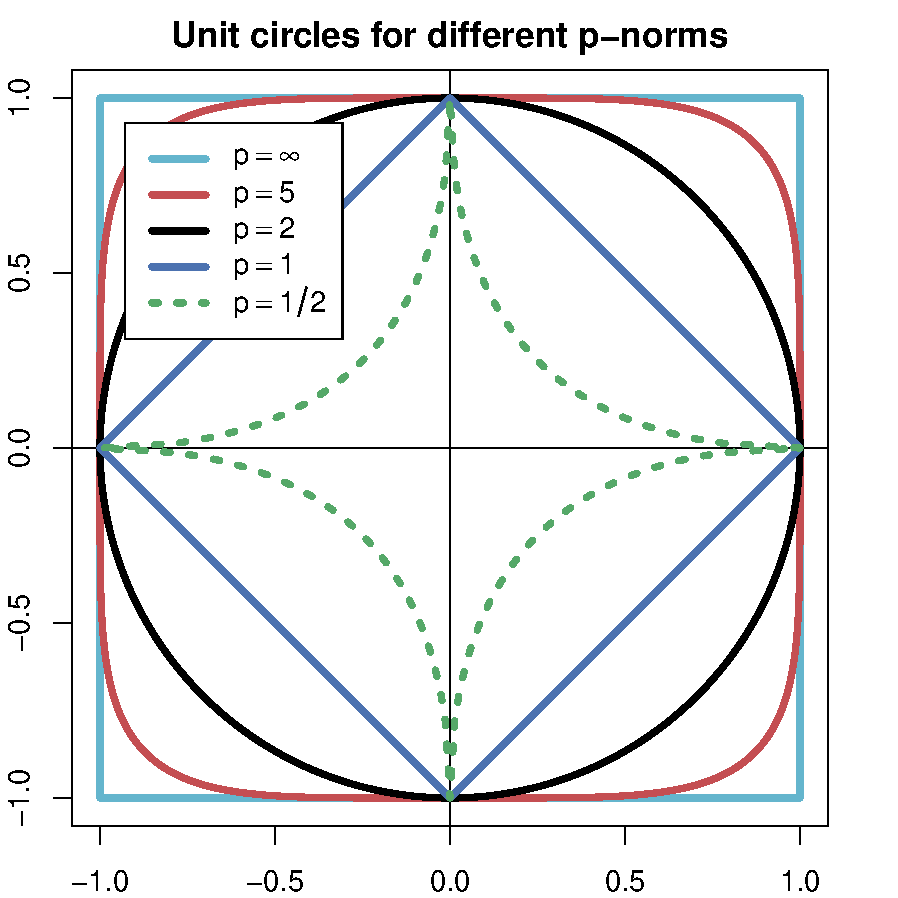
\includegraphics[width=55mm]{img/unit_circle_pnorms}%
%%     \end{column}
%%     \begin{column}{55mm}
%%       \begin{itemize}
%%        \item Visualisation of norms in $\setR^2$ by plotting \h{unit
%%            circle}, i.e.\ points $\vu$ with $\norm{\vu}=1$
%%        \item Here: $p$-norms $\norm[p]{\cdot}$ for different values of $p$%
%%        \item<2-> Triangle inequality $\iff$ unit circle is \h{convex}
%%        \item<2-> This shows that $p$-norms with $p < 1$ would violate the triangle
%%          inequality
%%       \end{itemize}
%%     \end{column}
%%   \end{columns}
%%   
%%   \gap[1]
%%   \begin{itemize}
%%   \item<3->[\hand] Consequence for DSM: $p \ll 2$ sensitive to small differences in many
%%     coordinates, $p \gg 2$ to larger differences in few coord.
%%   \end{itemize}
%% \end{frame}


%%%%%%%%%%%%%%%%%%%%%%%%%%%%%%%%%%%%%%%%%%
\subsection{Angles and orthogonality}

\begin{frame}
  \frametitle{Euclidean norm \& inner product}
  %% \framesubtitle{}

  \begin{itemize}
  \item The Euclidean norm $\norm[2]{\vu} = \sqrt{\vu^T \vu}$ is
    special because it can be derived from the \hh{inner product}:
    \[
    \vx^T \vy = x_1 y_1 + \dots + x_n y_n
    \]
  \item<2-> The inner product is a \secondary{positive definite} and \secondary{symmetric}
    \secondary{bilinear form} with an important geometric interpretation:
    \[
    \cos \phi = \frac{\vu^T \vv}{ \norm[2]{\vu}\cdot \norm[2]{\vv} }
    \]
    for the \h{angle} $\phi$ between vectors $\vu, \vv\in \setR^n$
    \begin{itemize}
    \item the value $\cos \phi$ is known as the \hh{cosine similarity} measure
    \end{itemize}
  \item<3-> In particular, $\vu$ and $\vv$ are \h{orthogonal} iff $\vu^T \vv = 0$
  \end{itemize}
\end{frame}


\begin{frame}[fragile]
  \frametitle{Cosine similarity in R}
  %% \framesubtitle{}

  \begin{itemize}
  \item Cosine similarities can be computed very efficiently if vectors are pre-normalized, so that $\norm[2]{\vu} = \norm[2]{\vv} = 1$
  \item[\hand] just need all inner products $\vm_i^T \vm_j$ between row vectors of $\mathbf{M}$
  \end{itemize}
  
  \onslide<2->
  \begin{small}
    \[
    \mathbf{M}\cdot \mathbf{M}^T = 
    \begin{bmatrix}
      \cdots & \vm_1 & \cdots \\
      \cdots & \vm_2 & \cdots \\
      \\
      \\
      \cdots & \vm_k & \cdots 
    \end{bmatrix}
    \cdot
    \begin{bmatrix}
      \vdots & \vdots & & \vdots \\
      \vm_1 & \vm_2 & & \vm_k \\
      \vdots & \vdots & & \vdots 
    \end{bmatrix}
    \]
  \end{small}
  \gap[.5]
  \[
  \text{\So}\quad
  \bigl( \mathbf{M}\cdot \mathbf{M}^T \bigr)_{ij}
  = \vm_i^T \vm_j
  \]

\begin{Rcode}
\REM{cosine similarities for row-normalized matrix:}
> sim <- tcrossprod(S0)
> angles <- acos(pmin(sim, 1)) * (180 / pi)
\end{Rcode}
\end{frame}

\begin{frame}[fragile]
  \frametitle{Euclidean distance or cosine similarity?}

  \begin{itemize}
  \item Proof that Euclidean distance and cosine similarity are equivalent looks much simpler in matrix algebra
  \item Assuming that $\norm[2]{\vu} = \norm[2]{\vv} = 1$, we have:
  \end{itemize}

  \onslide<2->\ungap[1]
  \begin{align*}
    \dist[2]{\vu}{\vv} 
    &= \norm[2]{\vu - \vv}
    = \sqrt{(\vu - \vv)^T (\vu - \vv)}
    \\
    &= \sqrt{\vu^T \vu + \vv^T \vv - 2\, \vu^T \vv}
    \\
    &= \sqrt{\norm[2]{\vu}^2 + \norm[2]{\vv}^2 - 2\, \vu^T \vv}
    \\
    &= \sqrt{2 - 2 \cos \phi}
  \end{align*}
  \ungap
  \begin{itemize}
  \item[\hand] $\dist[2]{\vu}{\vv}$ is a monotonically increasing function of $\phi$
  \end{itemize}
\end{frame}


%%%%%%%%%%%%%%%%%%%%%%%%%%%%%%%%%%%%%%%%%%%%%%%%%%%%%%%%%%%%%%%%%%%%%%
\section{Dimensionality reduction}

%%%%%%%%%%%%%%%%%%%%%%%%%%%%%%%%%%%%%%%%%%
\subsection{Orthogonal projection}

\begin{frame}
  \frametitle{Linear subspace \& basis}
  
  \begin{itemize}
  \item A linear \h{subspace} $B\subseteq \setR^n$ of rank $r\leq n$ is spanned by a set of $r$ linearly independent basis vectors
    \[
    B = \set{\vb_1, \ldots, \vb_r}
    \]
  \item<2-> Every point $\vu$ in the subspace is a unique linear combination of the basis vectors
    \[
    \vu = x_1 \vb_1 + \ldots + x_r \vb_r
    \]
    with coordinate vector $\vx\in \setR^r$
  \item<3-> Basis matrix $\mathbf{V} \in \setR^{n\times r}$ with column vectors $\vb_i$:
    \[
    \vu = \mathbf{V} \vx 
    \]
  \end{itemize}
\end{frame}

\begin{frame}
  \frametitle{Linear subspace \& basis}
  
  \begin{itemize}
  \item Basis matrix $\mathbf{V} \in \setR^{n\times r}$ with column vectors $\vb_i$:
    \[
    \vu = x_1 \vb_1 + \ldots + x_r \vb_r = \mathbf{V} \vx
    \]
  \end{itemize}

  \[
  \begin{array}{ccccc}
    \begin{bmatrix}
      x_1 b_{11} + \ldots + x_r b_{r1} \\
      x_1 b_{12} + \ldots + x_r b_{r2} \\
      \vdots\\
      x_1 b_{1n} + \ldots + x_r b_{rn}
    \end{bmatrix}
    & = &
    \begin{bmatrix}
      b_{11} & \cdots & b_{r1} \\
      b_{12} & \cdots & b_{r2} \\
      \vdots & & \vdots \\
      b_{1n} & \cdots & b_{rn}
    \end{bmatrix}
    & \cdot &
    \begin{bmatrix}
      x_1 \\
      \vdots \\
      x_r
    \end{bmatrix} \\
    \\
    \mathbf{u} & = & \mathbf{V} & \cdot & \mathbf{x} \\
    (n\times 1) & & (n\times \primary{r}) & & (\primary{r}\times 1)
  \end{array}
  \]

\end{frame}

\begin{frame}
  \frametitle{Orthonormal basis}

  \begin{itemize}
  \item Particularly convenient with orthonormal basis:
    \begin{align*}
      \norm[2]{\vb_i} &= 1 \\
      \vb_i^T \vb_j &= 0 && \text{for } i\neq j
    \end{align*}
  \item Corresponding basis matrix $\mathbf{V}$ is (column)-\hh{orthogonal}
    \[
      \mathbf{V}^T \mathbf{V} = \mathbf{I}_r
    \]
    and defines a \primary{Cartesian coordinate system} in the subspace
  \end{itemize}
\end{frame}

\begin{frame}
  \frametitle{The mathematics of projections}
  %% \framesubtitle{}

  \begin{columns}[c]
    \begin{column}{50mm}
      \begin{itemize}
      \item 1-d subspace spanned by basis vector
        $\norm[2]{\vb} = 1$
      \item For any point $\vu$, we have
        \[
          \cos \varphi
          = \frac{\vb^T \vu}{\norm[2]{\vb}\cdot \norm[2]{\vu}}
          = \frac{\vb^T \vu}{\norm[2]{\vu}}          
        \]
      \item<2-> Trigonometry: coordinate of point on the line is
        $x = \norm[2]{\vu}\cdot \cos\varphi = \vb^T \vu$
      \end{itemize}
    \end{column}
    \begin{column}{50mm}
      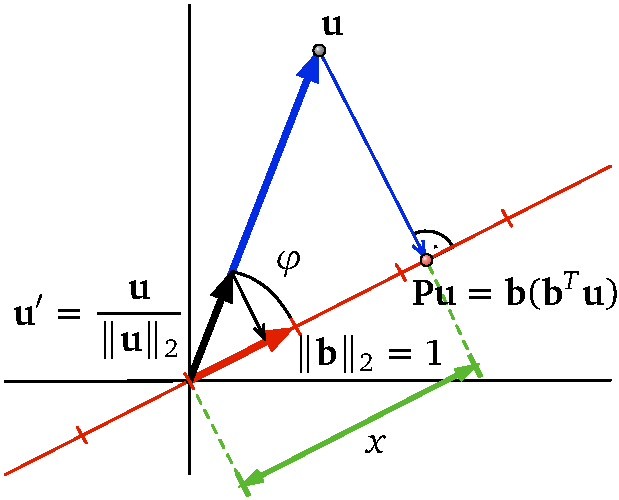
\includegraphics[width=50mm]{img/4_cosine_projection}
    \end{column}
  \end{columns}
  
  \begin{itemize}
  \item<3-> The projected point in original space is then given by
    \[
      \vb\cdot x = \vb (\vb^T \vu) = (\vb \vb^T) \vu = \mathbf{P} \vu
    \]
    where $\mathbf{P}$ is a \h{projection matrix} of rank 1
  \end{itemize}
\end{frame}


\begin{frame}
  \frametitle{The mathematics of projections}
  %% \framesubtitle{}

  \begin{itemize}
  \item For an orthogonal basis matrix $\mathbf{V}$ with columns
    $\vb_1, \ldots, \vb_r$, the projection into the rank-$r$ subspace $B$ is
    given by
    \[
      \mathbf{P}\vu = \left(\sum_{i=1}^r \vb_i \vb_i^T\right) \vu
      = \mathbf{V} \mathbf{V}^T \vu
    \]
    and its subspace coordinates are $\vx = \mathbf{V}^T \mathbf{u}$
  \item<2-> Projection can be seen as decomposition into the projected vector
    and its orthogonal complement
    \[
      \vu = \mathbf{P} \vu + (\vu - \mathbf{P} \vu)
      = \mathbf{P} \vu + (\mathbf{I} - \mathbf{P}) \vu
      = \mathbf{P} \vu + \mathbf{Q} \vu
    \]
  \item<3-> Because of orthogonality, this also applies to the squared
    Euclidean norm (according to the Pythagorean theorem)
    \[
      \norm{\vu}^2 = \norm{\mathbf{P} \vu}^2 + \norm{\mathbf{Q} \vu}^2
    \]
  \end{itemize}
\end{frame}

\begin{frame}[fragile]
  \frametitle{Aside: the matrix cross-product}

  \begin{itemize}
  \item We already know that the (transpose) cross-product $\mathbf{M} \mathbf{M}^T$
    computes all inner products between the row vectors of $\mathbf{M}$
    \begin{itemize}
    \item[]
    \end{itemize}
  \item But $\mathbf{V} \mathbf{V}^T$ it can also be unterstood as a \primary{superposition}
    of the \primary{outer products} of the columns of $\mathbf{V}$ with themselves
  \end{itemize}

  \gap[1]
  \begin{center}
    \begin{tikzpicture}[every matrix/.style={fixed matrix=6mm, cell matrix=5mm, matrix of nodes}]
      \matrix [nmatrix, anchor=north west]
      (vvt) at (0, 0) {
        {} \\
        $\mathbf{V} \mathbf{V}^T \; =$ \\
      } ;
      \matrix [bmatrix, below right={0mm and 4mm of vvt.north east}]
      (b1) {
        $b_{11}$ \\
        $\scaleVdots$ \\
        $b_{1n}$ \\
      } ;
      \matrix [nmatrix, below right={0mm and 0mm of b1.north east}] 
      (d1) {
        $\cdot$ \\
      } ;
      \matrix [bmatrix, below right={0mm and 0mm of d1.north east}] 
      (b1t) {
        $b_{11}$ & $\scaleCdots$ & $b_{1n}$ \\
      } ;
      \matrix [nmatrix, below right={0mm and 2mm of b1t.north east}] 
      (sum) {
        {} \\
        $+ \; \ldots \; +$ \\
      } ;
      \matrix [bmatrix, below right=(0mm and 4mm of sum.north east)]
      (br) {
        $b_{r1}$ \\
        $\scaleVdots$ \\
        $b_{rn}$ \\
      } ;
      \matrix [nmatrix, below right={0mm and 0mm of br.north east}] 
      (dr) {
        $\cdot$ \\
      } ;
      \matrix [bmatrix, below right={0mm and 0mm of dr.north east}] 
      (drt) {
        $b_{r1}$ & $\scaleCdots$ & $b_{rn}$ \\
      } ;
    \end{tikzpicture}
  \end{center}
\end{frame}

\begin{frame}[fragile]
  \frametitle{Projections in R}

  \begin{Rcode}
\REM{column basis vector for ``animal'' subspace}
> b <- t(t(c(1, 1, 1, 1, .5, 0, 0)))
> b <- normalize.cols(b) \REM{basis vectors must be normalized}

> (x <- M %*% b) \REM{projection of data points into subspace coordinates}
> x %*% t(b)     \REM{projected points in original space}
> tcrossprod(x, b) \REM{outer() only works for plain vectors}

> P <- b %*% t(b)  \REM{projection operator}
> P - t(P)         \REM{note that P is symmetric}
> M %*% P          \REM{projected points in original space}
\end{Rcode}

\end{frame}

\begin{frame}
  \frametitle{Optimal projections and subspaces}
  %% \framesubtitle{}

  \begin{itemize}
  \item Orthogonal decomposition of squared distances btw vectors
    \[
      \norm{\vu - \vv}^2 = \norm{\mathbf{P} \vu - \mathbf{P} \vv}^2 + \norm{\mathbf{Q} \vu - \mathbf{Q} \vv}^2
    \]
  \end{itemize}

  \begin{columns}[c]
    \begin{column}{60mm}
      \begin{itemize}
      \item<2-> Define projection \hh{loss} as difference btw squared distances
        \begin{align*}
          & \bigabs{\,\norm{\mathbf{P}(\vu - \vv)}^2 - \norm{\vu - \vv}^2\,} \\
          =\;& \norm{\vu - \vv}^2 - \norm{\mathbf{P}(\vu - \vv)}^2 \\
          =\;& \norm{\mathbf{Q}(\vu - \vv)}^2
        \end{align*}
      \item<3-> Projection quality measure:
        \[
          R^2 = \frac{\norm{\mathbf{P}(\vu - \vv)}^2}{\norm{\vu - \vv}^2}
        \]
      \end{itemize}
    \end{column}
    \begin{column}{40mm}
      \hspace*{-5mm}%
      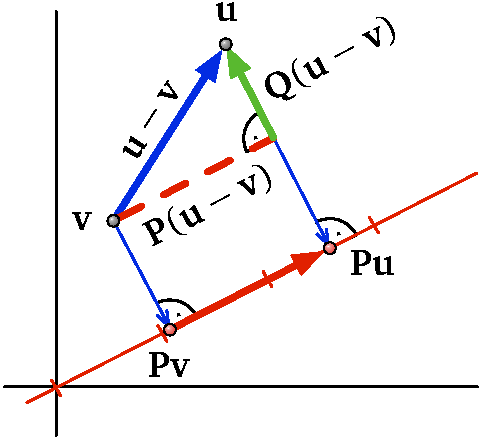
\includegraphics[width=45mm]{img/4_projection_loss}      
    \end{column}
  \end{columns}
\end{frame}

\begin{frame}
  \frametitle{Optimal projections and subspaces}

  \begin{itemize}
  \item Optimal subspace maximises $R^2$ across a data set $\mathbf{M}$,
    which is now specified in terms of row vectors $\vm_i^T$:
    \begin{align*}
      \vx_i^T &= \vm_i^T \mathbf{V}
      & \vm_i^T \mathbf{P} &= \vm_i^T \mathbf{V} \mathbf{V}^T \\
      \mathbf{X} &= \mathbf{M} \mathbf{V}
      & \mathbf{M} \mathbf{P} &= \mathbf{M} \mathbf{V} \mathbf{V}^T
    \end{align*}
  \item<2-> We will now show that the overall projection quality is
    \[
      R^2 = \frac{\sum_{i=1}^k \norm{\vm_i^T \mathbf{P}}^2}{\sum_{i=1}^k \norm{\vm_i^T}^2}
      = \frac{\norm[F]{\mathbf{M} \mathbf{P}}^2}{\norm[F]{\mathbf{M}}^2}
    \]
    with the (squared) \hh{Frobenius norm} \ungap
    \[
      \norm[F]{\mathbf{M}}^2 = \sum_{ij} (m_{ij})^2 = \sum_{i=1}^k \norm{\vm_i}^2
    \]
  \end{itemize}
\end{frame}

\newcommand{\sumij}[1][i,\,j]{\textstyle\sum_{{#1} = 1}^k}
\begin{frame}
  \frametitle{Optimal projections and subspaces}

  \begin{itemize}
  \item For a \primary{centered} data set with $\sum_i \vm_i = \vnull$, the Frobenius norm
    corresponds to the average (squared) distance between points
  \end{itemize}

  \ungap[1.5]
  \begin{align*}
    \sumij & \norm{\vm_i - \vm_j}^2 \\
    \visible<2->{
           &= \sumij (\vm_i - \vm_j)^T (\vm_i - \vm_j) }\\
    \visible<3->{
           &= \sumij \bigl( \norm{\vm_i}^2 + \norm{\vm_j}^2 - 2 \vm_i^T \vm_j \bigr) }\\
    \visible<4->{
           &= \sumij[j] \norm[F]{\mathbf{M}}^2
             + \sumij[i] \norm[F]{\mathbf{M}}^2
             - 2 \sumij[i] \vm_i^T \bigl( \secondary{\underbrace{\sumij[j] \vm_j}_{\vnull}} \bigr) }\\
    \visible<5->{
           &= 2k \cdot \norm[F]{\mathbf{M}}^2 }
  \end{align*}

  \begin{itemize}
  \item<6-> Similarly for the overall projection loss and quality $R^2$:
    \[
      R^2 = 
      \frac{
        \sumij \norm{\mathbf{P}(\vm_i - \vm_j)}^2
      }{
        \sumij \norm{\vm_i - \vm_j}^2
      }
      = \frac{
        2k \cdot \norm[F]{\mathbf{M} \mathbf{P}}^2
      }{
        2k \cdot \norm[F]{\mathbf{M}}^2
      }
    \]
  \end{itemize}
\end{frame}

%%%%%%%%%%%%%%%%%%%%%%%%%%%%%%%%%%%%%%%%%%
\subsection{PCA \& SVD}

\begin{frame}
  \frametitle{Singular value decomposition}
  %% \framesubtitle{}

  \ungap[1]
  \begin{itemize}
  \item Fundamental result of matrix algebra: \h{singular value decomposition}
    (\hh{SVD}) factorises any matrix $\mathbf{M}$ into
    \[
    \mathbf{M} = \mathbf{U} \Msigma \mathbf{V}^T
    \]
    where $\mathbf{U}$ and $\mathbf{V}$ are orthogonal and $\Msigma$ is a diagonal matrix of
    \hh{singular values} $\sigma_1\geq \sigma_2\geq \dots \geq \sigma_m > 0$
  \end{itemize}

  \begin{equation*}
    \begin{bmatrix}
      & & \primary{n} & & \\
      & & & & \\
      & & & & \\
      \primary{k} & & \mathbf{M} & & \\
      & & & & \\
      & & & & \\
      & & & & 
    \end{bmatrix}
    =
    \begin{bmatrix}
      & & & \primary{m} & & & \\
      & & & & & & \\
      & & & & & & \\
      \primary{k} & & & \mathbf{U} & & & \\
      & & & & & & \\
      & & & & & & \\
      & & & & & &
    \end{bmatrix}
    \cdot
    \begin{bmatrix}
      \sigma_1 & \primary{m} & \\
      \primary{m} & \ddots & \\
      & \Msigma & \sigma_m
    \end{bmatrix}
    \cdot
    \begin{bmatrix}
      & & \primary{n} & & \\
      & & & & \\
      \primary{m} & & \mathbf{V}^T & & \\
      & & & & \\
      & & & &
    \end{bmatrix}
  \end{equation*}
\end{frame}

\begin{frame}
  \frametitle{Singular value decomposition}

  \begin{itemize}
  \item $m \leq \min \set{k, n}$ is the inherent dimensionality (\hh{rank}) of $\mathbf{M}$
  \item Columns $\va_i$ of $\mathbf{U}$ are called left singular vectors,\\
    columns $\vb_i$ of $\mathbf{V}$ (= rows of $\mathbf{V}^T$) are right singular vectors
  \item<2-> Recall the ``outer product'' view of matrix multiplication:
    \[
      \mathbf{U} \mathbf{V}^T = \sum_{i=1}^m \va_i \vb_i^T
    \]
  \item<3-> Hence the SVD corresponds to a sum of rank-1 components
    \[
      \mathbf{M} = \mathbf{U} \Msigma \mathbf{V}^T = \sum_{i=1}^m \sigma_i \va_i \vb_i^T
    \]
  \end{itemize}
\end{frame}

\begin{frame}
  \frametitle{Singular value decomposition}

  \begin{itemize}
  \item Key property of SVD: the first $r$ components give the best rank-$r$
    approximation to $\mathbf{M}$ with respect to the Frobenius norm, i.e.\ they minimize the loss
    \[
      \norm[F]{ \mathbf{U}_r \Msigma_r \mathbf{V}_r^T - \mathbf{M} }^2
      = \norm[F]{ \mathbf{M}_r - \mathbf{M} }^2
    \]
  \item[\hand] \hh{Truncated} SVD
    \begin{itemize}
    \item $\mathbf{U}_r$, $\mathbf{V}_r$ = first $r$ columns of $\mathbf{U}$, $\mathbf{V}$
    \item $\Msigma_r$ = diagonal matrix of first $r$ singular values
    \end{itemize}
  \item<2-> It can be shown that
    \[
      \norm[F]{ \mathbf{M} }^2 = \sum_{i=1}^m \sigma_i^2 \quad \text{and} \quad
      \norm[F]{ \mathbf{M}_r }^2 = \sum_{i=1}^r \sigma_i^2      
    \]
  \end{itemize}
\end{frame}

\begin{frame}
  \frametitle{SVD dimensionality reduction}

  \begin{itemize}
  \item Columns of $\mathbf{V}_r$ form an orthogonal basis of the optimal rank-$r$ subspace because
    \[
      \mathbf{M} \mathbf{P} = \mathbf{M} \mathbf{V}_r \mathbf{V}_r^T
      = \mathbf{U} \Msigma \secondary{\underbrace{\mathbf{V}^T \mathbf{V}_r}_{= \mathbf{I}_r}} \mathbf{V}_r^T
      = \mathbf{U}_r \Msigma_r \mathbf{V}_r^T = \mathbf{M}_r
    \]
  \item<2-> \h{Dimensionality reduction} uses the subspace coordinates
    \[
      \mathbf{M} \mathbf{V}_r = \mathbf{U}_r \Msigma_r
    \]
  \item<3-> If $\mathbf{M}$ is centered, this also gives the best possible
    preservation of pairwise distances \so \primary{principal component analysis}
    (\hh{PCA})
    \begin{itemize}
    \item[\hand] but centering is usally omitted in order to maintain sparseness,
      so SVD preserves vector lengths rather than distances
    \end{itemize}
  \end{itemize}
\end{frame}

\begin{frame}
  \frametitle{Scaling SVD dimensions}

  \begin{itemize}
  \item Singular values $\sigma_i$ can be seen as weighting of the latent
    dimensions, which determines their contribution to
    \[
      \norm[F]{\mathbf{M} \mathbf{V}_r} = \sigma_1^2 + \ldots + \sigma_r^2
    \]
  \item<2-> Weighting adjusted by \h{power scaling} of the singular values:
    \[
      \mathbf{U}_r \Msigma_r^p
      = \begin{bmatrix}
        \vdots &  & \vdots \\
        \sigma_1^p \va_1 & \cdots & \sigma_r^p \va_r \\
        \vdots &  & \vdots 
      \end{bmatrix}
    \]
    \ungap[1]
    \begin{itemize}
    \item $p = 1$: normal SVD projection
    \item $p = 0$: dimension weights equalized
    \item $p = 2$: more weight given to first latent dimensions
    \end{itemize}
  \item<2-> Other weighting schemes possible (e.g.\ skip first dimensions)
  \end{itemize}
\end{frame}

\newcommand{\Szero}{\ensuremath{\mathbf{S}_0}}
\newcommand{\sigmaSeven}{\ensuremath{\sigma_7}}
\newcommand{\Rsquared}{\ensuremath{R^2}}
\begin{frame}[fragile]
  \frametitle{SVD projection in R}

\begin{Rcode}
> fact <- svd(S0)     \REM{SVD decomposition of \Szero}
> round(fact$u, 3)    \REM{left singular vectors (columns) = \(\mathbf{U}\)}
> round(fact$v, 3)    \REM{right singular vectors (columns) = \(\mathbf{V}\)}
> round(fact$d, 3)    \REM{singular values = diagonal of \(\Msigma\)}
\REM{note that \Szero{} has effective rank 6 because \(\sigmaSeven \approx 0\)}
> barplot(fact$d ^ 2) \REM{\Rsquared{} contributions}

> r <- 2              \REM{truncated rank-2 SVD}
> (U.r <- fact$u[, 1:r])
> (Sigma.r <- diag(fact$d[1:r], nrow=r))
> (V.r <- fact$v[, 1:r])
\end{Rcode}
\end{frame}

\begin{frame}[fragile]
  \frametitle{SVD projection in R}
  
\begin{Rcode}
> (X.r <- S0 %*% V.r) \REM{project into latent coordinates}
> U.r %*% Sigma.r     \REM{same result}
> scaleMargins(U.r, cols=fact$d[1:r]) \REM{the \texttt{wordspace} way}

> rownames(X.r) <- rownames(S0)       \REM{NB: keep row labels}

> S0r <- U.r %*% Sigma.r %*% t(V.r)   \REM{rank-2 matrix approx.}
> round(S0r, 3)
\REM{compare with \Szero: where are the differences?}

> round(X.r %*% t(V.r), 3)            \REM{same result}
\end{Rcode}

\begin{itemize}
\item[\hand] see example code for comparison against PCA with centering
\end{itemize}
\end{frame}


%%%%%%%%%%%%%%%%%%%%%%%%%%%%%%%%%%%%%%%%%%%%%%%%%%%%%%%%%%%%%%%%%%%%%%
%% \section{}

%%%%%%%%%%%%%%%%%%%%%%%%%%%%%%%%%%%%%%%%%%
%% \subsection{}


%%%%%%%%%%%%%%%%%%%%%%%%%%%%%%%%%%%%%%%%%%%%%%%%%%%%%%%%%%%%%%%%%%%%%%
%% References (if any)

% \frame[allowframebreaks]{
%   \frametitle{References}
%   \bibliographystyle{natbib-stefan}
%   \begin{scriptsize}
%     \bibliography{dsm}
%   \end{scriptsize}
% }

\end{document}
